\documentclass{tufte-handout}

\title{Section 5.5: Inverse Trigonometric Functions and Their Graphs}

\author[AW]{Ammon Washburn}

\usepackage{graphicx} % allow embedded images
  \setkeys{Gin}{width=\linewidth,totalheight=\textheight,keepaspectratio}
  \graphicspath{{graphics/}} % set of paths to search for images
\usepackage{amsmath}  % extended mathematics
\usepackage{booktabs} % book-quality tables
\usepackage{units}    % non-stacked fractions and better unit spacing
\usepackage{multicol} % multiple column layout facilities
\usepackage{lipsum}   % filler text
\usepackage{enumerate}
\usepackage{wrapfig}
\usepackage{fancyvrb} % extended verbatim environments
  \fvset{fontsize=\normalsize}% default font size for fancy-verbatim environments
\usepackage{tikz}
\usepackage{subcaption}
\captionsetup{compatibility=false}
\usepackage{mathtools}
\usepackage{graphicx}
\usepackage{amssymb}
\usepackage{enumerate}
\usepackage{color}
\usepackage{fancyvrb}
\usepackage{breqn}
\usepackage{fancyhdr}
\usepackage{multicol}
%\usepackage[latin1]{inputenc}
\usepackage{tikz}
\usepackage{pgfplots}
\pgfplotsset{compat=1.8}

\definecolor{dkgreen}{rgb}{0,0.6,0}
\definecolor{gray}{rgb}{0.5,0.5,0.5}
\definecolor{mauve}{rgb}{0.58,0,0.82}

\newcommand{\R}[1]{\mathbb{R}^{#1}}

\pgfplotsset{vasymptote/.style={
    before end axis/.append code={
        \draw[densely dashed] ({rel axis cs:0,0} -| {axis cs:#1,0})
        -- ({rel axis cs:0,1} -| {axis cs:#1,0});
    }
}}
\pgfplotsset{hasymptote/.style={
    before end axis/.append code={
    	%\draw (axis cs:0,1) -- ({axis cs:0,1}-|{rel axis cs:1,0});
        \draw[densely dashed] ({rel axis cs:0,1} -| {axis cs:0,#1})
        -- ({rel axis cs:0,0} -| {axis cs:0,#1});
    }
}}

% Standardize command font styles and environments
\newcommand{\doccmd}[1]{\texttt{\textbackslash#1}}% command name -- adds backslash automatically
\newcommand{\docopt}[1]{\ensuremath{\langle}\textrm{\textit{#1}}\ensuremath{\rangle}}% optional command argument
\newcommand{\docarg}[1]{\textrm{\textit{#1}}}% (required) command argument
\newcommand{\docenv}[1]{\textsf{#1}}% environment name
\newcommand{\docpkg}[1]{\texttt{#1}}% package name
\newcommand{\doccls}[1]{\texttt{#1}}% document class name
\newcommand{\docclsopt}[1]{\texttt{#1}}% document class option name
\newenvironment{docspec}{\begin{quote}\noindent}{\end{quote}}% command specification environment
\newcommand{\Z}[1]{\mathbb{Z}^{#1}}

\newtheorem{mydef}{Definition}
\providecommand{\floor}[1]{\left \lfloor #1 \right \rfloor }
\providecommand{\abs}[1]{| #1 |}


\begin{document}

\begin{abstract}
Learn how to restrict sine and cosine to get 1-1 functions
\end{abstract}

\section{The Inverse Sine Function}
Need to restrict domain of sine so that it passes the horizontal line test. \\
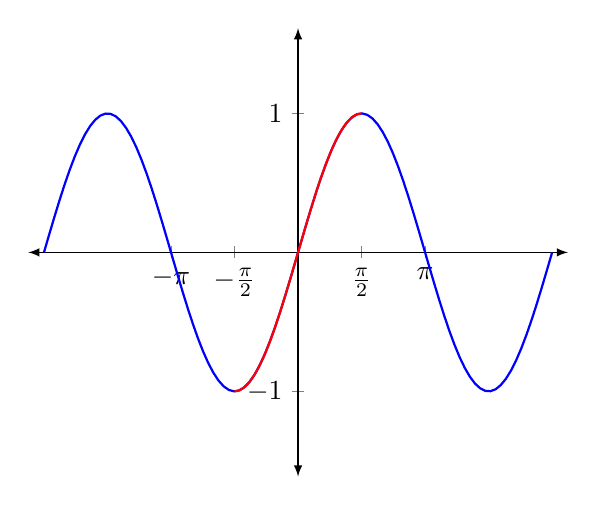
\begin{tikzpicture}
\begin{axis}[
    %axis equal image,
    axis lines=middle,
    xmin=-2*pi,xmax=2*pi,
    ymin=-1.5,ymax=1.5,
    enlargelimits={abs=0.2cm},
    axis line style={latex-latex},
    ticklabel style={fill=white},
    ytick={-1, 1},
    xtick={-3.14, -1.57, 1.57, 3.14},
    xticklabels={$-\pi$, $-\frac{\pi}{2}$, $\frac{\pi}{2}$, $\pi$},
]
	% Draw the two parts separately with individual domains:
	\addplot[samples=100,domain=-2*pi:2*pi, thick, color=blue] {sin(deg(x))};
	\addplot[samples=50, domain=-pi/2:pi/2, thick, color=red] {sin(deg(x))};
\end{axis}
\end{tikzpicture} \\
\textbf{Def:} The \textbf{inverse sine function} with domain [-1, 1] and range $[-\pi/2, \pi/2]$ is defined as
\begin{align*}
\sin^{-1}(x) = y \Leftrightarrow x = \sin(y)
\end{align*}
also called \textbf{arcsine}, denoted $\arcsin$. \\
\textbf{Cancellation properties:} 
\begin{align*}
\sin(\sin^{-1}(x)) = x &\qquad\text{for } -1 \leq x \leq 1 \\
\sin^{-1}(\sin(x)) = x &\qquad\text{for } -\frac{\pi}{2} \leq x \leq \frac{\pi}{2}
\end{align*}

\subsection{Examples}
\begin{enumerate}
\item $\sin^{-1}(-1/2)$ {\color{blue} $-\pi/6$}
\item $\sin^{-1}(\pi/2)$ {\color{blue} undefined, since $\pi/2 > 1$}
\item $\sin^{-1}(0.82)$ {\color{blue} $\approx 0.96141$ (use calc)}
\item $\sin^{-1}\left( \sin\left(\frac{2\pi}{3} \right) \right)$ {\color{blue} $= \frac{\pi}{3}$, since $2\pi/3$ not in interval}
\end{enumerate}

\section{The Inverse Cosine Function}
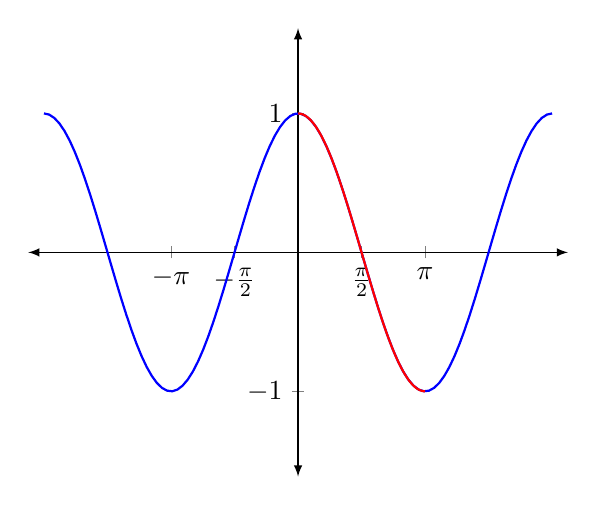
\begin{tikzpicture}
\begin{axis}[
    %axis equal image,
    axis lines=middle,
    xmin=-2*pi,xmax=2*pi,
    ymin=-1.5,ymax=1.5,
    enlargelimits={abs=0.2cm},
    axis line style={latex-latex},
    ticklabel style={fill=white},
    ytick={-1, 1},
    xtick={-3.14, -1.57, 1.57, 3.14},
    xticklabels={$-\pi$, $-\frac{\pi}{2}$, $\frac{\pi}{2}$, $\pi$},
]
	% Draw the two parts separately with individual domains:
	\addplot[samples=100,domain=-2*pi:2*pi, thick, color=blue] {cos(deg(x))};
	\addplot[samples=50, domain=0:pi, thick, color=red] {cos(deg(x))};
\end{axis}
\end{tikzpicture} \\
\textbf{Def:} The \textbf{inverse cosine function} with domain [-1, 1] and range $[0, \pi]$ is defined as
\begin{align*}
\cos^{-1}(x) = y \Leftrightarrow x = \cos(y)
\end{align*}
also called \textbf{arccosine}, denoted $\arccos$. \\
\textbf{Cancellation properties:} 
\begin{align*}
\cos(\cos^{-1}(x)) = x &\qquad\text{for } -1 \leq x \leq 1 \\
\cos^{-1}(\cos(x)) = x &\qquad\text{for } 0 \leq x \leq \pi
\end{align*}

\subsection{Examples}
\begin{enumerate}
\item $\cos^{-1}(\sqrt{3}/2)$ {\color{blue} $\pi/6$}
\item $\cos^{-1}(5/7)$ {\color{blue} $\approx 0.77519$ (use calc)}
\item $\cos^{-1}\left( \cos\left(\frac{2\pi}{3} \right) \right)$ {\color{blue} $= \frac{2\pi}{3}$, since $2\pi/3$ is in interval}
\end{enumerate}

\section{The Inverse Tangent Function}
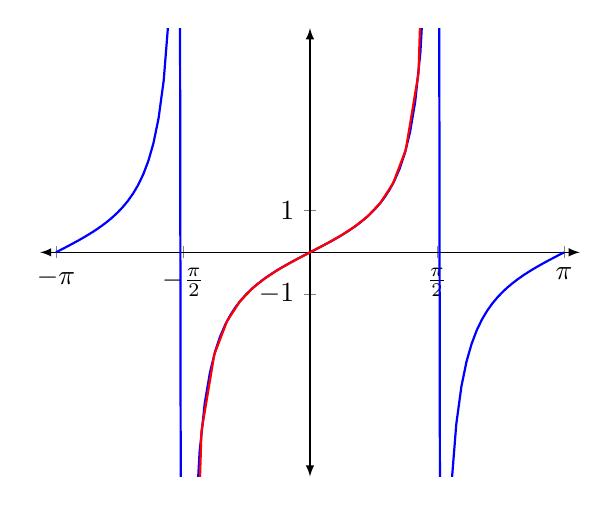
\begin{tikzpicture}
\begin{axis}[
    %axis equal image,
    axis lines=middle,
    xmin=-pi,xmax=pi,
    ymin=-5,ymax=5,
    enlargelimits={abs=0.2cm},
    axis line style={latex-latex},
    ticklabel style={fill=white},
    ytick={-1, 1},
    xtick={-3.14, -1.57, 1.57, 3.14},
    xticklabels={$-\pi$, $-\frac{\pi}{2}$, $\frac{\pi}{2}$, $\pi$},
]
	% Draw the two parts separately with individual domains:
	\addplot[samples=100,domain=-pi:pi, thick, color=blue] {tan(deg(x))};
	\addplot[samples=20, domain=-1.5:1.5, thick, color=red] {tan(deg(x))};
\end{axis}
\end{tikzpicture} \\
\textbf{Def:} The \textbf{inverse tangent function} with domain $[-\infty, \infty]$ and range $(-\pi/2, \pi/2)$ is defined as
\begin{align*}
\tan^{-1}(x) = y \Leftrightarrow x = \tan(y)
\end{align*}
also called \textbf{arctangent}, denoted $\arctan$. \\
\textbf{Cancellation properties:} 
\begin{align*}
\tan(\tan^{-1}(x)) = x &\qquad \text{for } x\in \R{} \\
\tan^{-1}(\tan(x)) = x &\qquad \text{for } -\frac{\pi}{2} < x < \frac{\pi}{2}
\end{align*}

\subsection{Examples}
\begin{enumerate}
\item $\tan^{-1}(1)$ {\color{blue} $\pi/4$}
\item $\tan^{-1}(20)$ {\color{blue} $\approx 1.52084$ (use calc)}
\item $\tan^{-1}(\tan(4\pi))$ {\color{blue} $= 0$, since $4\pi$ not in interval}
\item $\tan(\tan^{-1}(20))$ {\color{blue} $= 20$, since $20$ is in interval}
\end{enumerate}

\section{More Examples}
\begin{enumerate}
\item $\tan(\sin^{-1}(1/2))$ {\color{blue} $= \tan(\pi/6) = \sqrt{3}/3$}
\item $\cos(\sin^{-1}(0))$ {\color{blue} $= \cos(0) = 1$}
\item $\cos(\sin^{-1}(x))$ {\color{blue} $ = \sqrt{1-x^2}$ (draw unit circle and stuff)}
\end{enumerate}

\end{document}